\documentclass[12pt, a4paper]{report}

\usepackage{ngerman}
\usepackage[utf8]{inputenc}

\usepackage{tipa}
\usepackage{here} 

%\usepackage[T1]{fontenc}

\usepackage{comment}

\usepackage{listings} 

\usepackage{blindtext}
\usepackage{fancyhdr} %Fuer Kopf und Fusszeilen
\usepackage{anysize} %Damit man Raender leicht einstellen kann
\usepackage{titlesec}

\usepackage{bookmark,hyperref}

\usepackage{tabularx}
\usepackage{rotating}
\usepackage{hhline}

%\usepackage{float}
\usepackage{floatrow}
%\usepackage[sc,center]{titlesec} %Um Kapitelnamen-Schrift zu veraendern
%\usepackage[T1]{fontenc} %ueblich
\usepackage{subfigure}

%\renewcommand{\thesubfigure}{\thefigure.\arabic{subfigure}}
%\makeatletter
%\renewcommand{\p@subfigure}{}
%\renewcommand{\@thesubfigure}{\thesubfigure:\hskip\subfiglabelskip}
%\makeatother

%\makeindex

%Paket zum importieren von Bildern
\usepackage{graphicx}
\newcommand{\HRule}{\rule{\linewidth}{0.2mm}}
\usepackage{tikz}
\usetikzlibrary{trees}

\usepackage{pageslts}
\usepackage{thumbs}
\usepackage{hyperref}

\usepackage{tabularx}

\usepackage{wrapfig} % Paket zur Positionierung einbinden

\usepackage{bibgerm}

\usepackage{amssymb} % Mathe Symbole
\usepackage{amsmath} % Mathe

\usepackage{booktabs}
\usepackage{subfigure}

\usepackage[nottoc]{tocbibind}

%Zeilenabstand ist jetzt 1.5 fach
\usepackage{setspace}
\onehalfspacing 
%Bilder werden auch im Unterverzeichnis img gesucht
\graphicspath{{img/}} 

\usepackage[Algorithmus]{algorithm}
\usepackage{algorithmic}

%Raender
%\marginsize{3.5cm}{1.5cm}{2.5cm}{2.5cm}
%\marginsize{3.5cm}{1.75cm}{2.5cm}{2.25cm}

\definecolor{haw_rot}{RGB}{160,0,0}
\definecolor{lgrey}{RGB}{240,240,240}


\newcommand{\mytoprule}{\specialrule{0.12em}{0em}{0em}}
\newcommand{\mybottomrule}{\specialrule{0.12em}{0em}{0em}} 
\renewcommand{\arraystretch}{1.2}

\usepackage{placeins}

%\renewcommand{\thesubfigure}{\thefigure.\arabic{subfigure}}
%\makeatletter
%\renewcommand{\p@subfigure}{}
%\renewcommand{\@thesubfigure}{\thesubfigure:\hskip\subfiglabelskip}
%\makeatother

%\makeindex
\usepackage{courier}
\lstset{ basicstyle=\small\ttfamily,
		 breaklines=true,}

\hyphenation{
}
\begin{document}


%pagenumbering wird benoetigt um Warnung zu beheben.
%wird wieder ueberschrieben
\pagenumbering{Roman}
\begin{titlepage}


\begin{center}


% Upper part of the page
%\begin{flushleft}
%
\includegraphics[angle=0,width=10cm]{./img/HL_WBM_de_B_300dpi.jpg}\\[3cm]    
%\end{flushleft}

%\textsc{\LARGE Hochschule Landshut}\\[1.5cm]

\includegraphics[angle=0,width=7cm]{./img/HL_WBM_de_B_300dpi.jpg}\\[2cm]


\textsc{\LARGE Masterarbeit}\\[0.6cm]

\small 

am Labor für medizinische Bildverarbeitung, Algorithmen und Krankenhaus IT \\[1cm]
zur Erlangung des akademischen Grades\\
\textbf{Master of Science (M. Sc.)} \\[1cm]

\normalsize

% Title
\HRule \\[0.4cm]
{
	
	\bfseries Entwicklung einer modularen und erweiterbaren Anwendung \\
	 zur medizinischen Bildverarbeitung
}\\[0.4cm]
\HRule \\[1.3cm]






%{\large \today}

\vfill

\footnotesize 

\begin{tabularx}{\textwidth}{Xr}
  \textbf{eingereicht von} 	& 	Rudolf Franz Siegfried Korb, 790060 \\ 
  \textbf{Erstprüfer} 		& 	Prof., Dr. Holger Timinger \\ 
  \textbf{Zweitprüferin} 	& 	Prof., Dr. Gudrun Schiedermeier \\ 
  \textbf{Abgabetermin}		&	02.03.2014
\end{tabularx}

\end{center}

%Bottom of page
% Author and supervisor
%\begin{minipage}{0.4\textwidth}
%\begin{flushleft} 
%\emph{Autor:}\\
%Rudolf Korb
%\end{flushleft}
%\end{minipage}
%\hfill
%\begin{minipage}{0.4\textwidth}
%\begin{flushright} 
%\emph{Betreuer:} \\
%Prof., Dr. Holger Timinger \\
%Prof., Dr. Gudrun Schiedermeier
%\end{flushright}
%\end{minipage}





\end{titlepage}

\pagestyle{empty}
% Das folgende braucht man, damit auch wirklich 1 Leerseite gelassen wird
\mbox{}
\clearpage

%Veraendert die Seitennummerierung zu roemischen Zeichen...
\setcounter{page}{1}

\renewcommand{\thepage}{\roman{page}}
%\pagestyle{headings}

\tableofcontents


\pagebreak

\renewcommand{\thepage}{\arabic{page}}
\setcounter{page}{1}

%Thumbverzeichnis
\addthumbsoverviewtocontents{chapter}{Kapitelübersicht}%Schreibt die Kapitelübersicht als Kapitel ins TOC
\thumbsoverview{Kapitelübersicht} 

\pagestyle{fancy} %eigener Seitenstil
\fancyhf{} %alle Kopf- und Fußzeilenfelder bereinigen
\renewcommand{\chaptermark}[1]{ \markboth{#1}{} }
\fancyhead[L]{\leftmark} %Kopfzeile links
%\fancyhead[C]{} %zentrierte Kopfzeile
%\fancyhead[R]{} %Kopfzeile rechts

%\fancyhead[R]{\textit{ \nouppercase{\leftmark}} }
%\fancyhead[L]{\textit{ \nouppercase{\rightmark}} }

\renewcommand{\headrulewidth}{0.3pt} %obere Trennlinie
\fancyfoot[C]{\thepage} %Seitennummer
\renewcommand{\footrulewidth}{0.3pt} %untere Trennlinie


\chapter{Einleitung}\label{einleitung}
\addthumb{Einleitung}{\huge{\textbf{\thechapter.}}}{white}{haw_rot} 

Ziel dieser Abschlussarbeit ist die Entwicklung einer Software zur medizinischen Bildverarbeitung. Eine modulare und flexible Architektur soll eine leichte Erweiterbarkeit sowohl für Entwickler (Erstellen eigener Werkzeuge) als auch den Anwender (Integration selbst implementierter Bildverarbeitungsalgorithmen) ermöglichen.\\
Das Programm soll für Forschung und Lehre am Labor für medizinische Bildverarbeitung, Algorithmen und Krankenhaus IT eingesetzt werden. Nach einer Vorstellung des Labors und dem zugehörigen Studiengang der biomedizinischen Technik erfolgt die Analyse der Anforderungen der Software. Aufbauend werden einige Grundlagen zur medizinischen Bildverarbeitung dargestellt. Der Fokus liegt auf dem DICOM-Standard und den Eigenschaften der medizinischen Bilddaten. Das nächste Kapitel erläutert die Softwarearchitektur sowie die Implementierung. Praktische Anwendungsbeispiele schließen die technischen Aspekte der Arbeit ab. Die folgende Diskussion zeigt Erweiterungsmöglichkeiten für die zukünftige Entwicklung auf.

\section{Der sechste Kondratieff-Zyklus}
Im Jahr 1926 veröffentlichte der Wirtschaftswissenschaftler Nikolai D. Kondratieff (* 1892, \dag 1938) die Theorie \glqq Die Langen Wellen der Konjunktur\grqq\ \cite{hensen:gesundeGesellschaft}.
Leo Nefiodow erweiterte 2006 die Theorie, damit die Entwicklung des 20. Jahrhunderts einfließen konnte.\\
Kondratieff zeigte, dass sich die gesellschaftliche Wandlung nicht willkürlich vollzog. Seit der Industrialisierung Mitte des 18. Jahrhunderts stand der Wohlstand der Gesellschaft in direkter Beziehung zu besonderen Erfindungen. Er betrachtete die Phasen des Wohlstandes und die direkt folgende Wirtschaftskrise und entdeckte die später nach ihm benannten \glqq Kondratieff-Zyklen\grqq\.
Wie in Abbildung \ref{zyklen} zu sehen ist, war die Dampfmaschine die erste Basisinnovation\footnote{Basisinnovationen müssen nach Nefiodow vier Eigenschaften erfüllen: Entstehung eines neuen Marktes mit vielen Arbeitsplätzen; Innovation bestimmt den Zyklus; Basisinnovationen haben einen Zyklus von 40 - 60 Jahren; Sie bestimmen die Entwicklungsrichtung} und revolutionierte die Textilindustrie.\cite{wieden:liquidwork}

%\begin{wrapfigure}{c}{10cm}
%\centering
%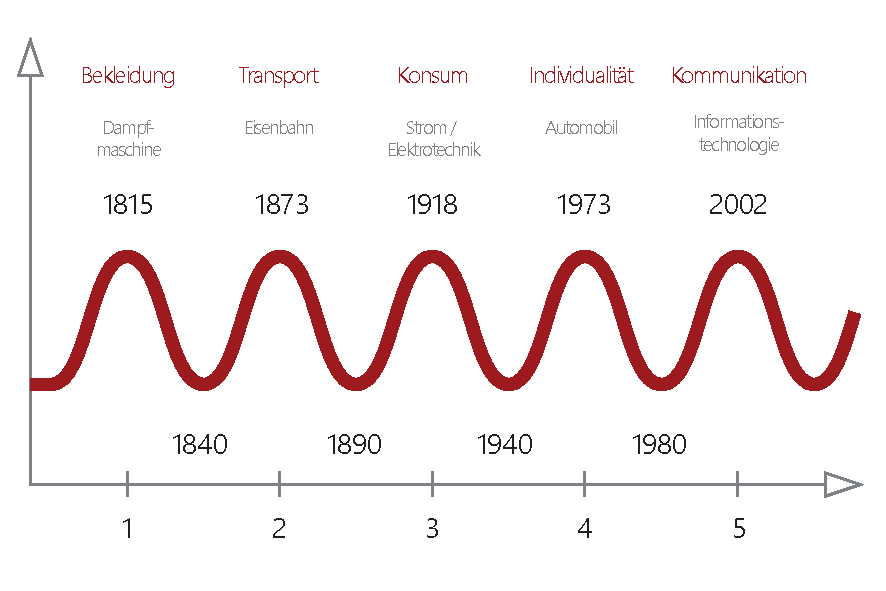
\includegraphics[width=8cm]{./img/zyklen.pdf}
%\caption{Kontratieff Zyklen}
%\label{zyklen}
%\end{wrapfigure}

\begin{figure}[htbp]
  \vspace{0.5cm}
  \centering
  \fbox{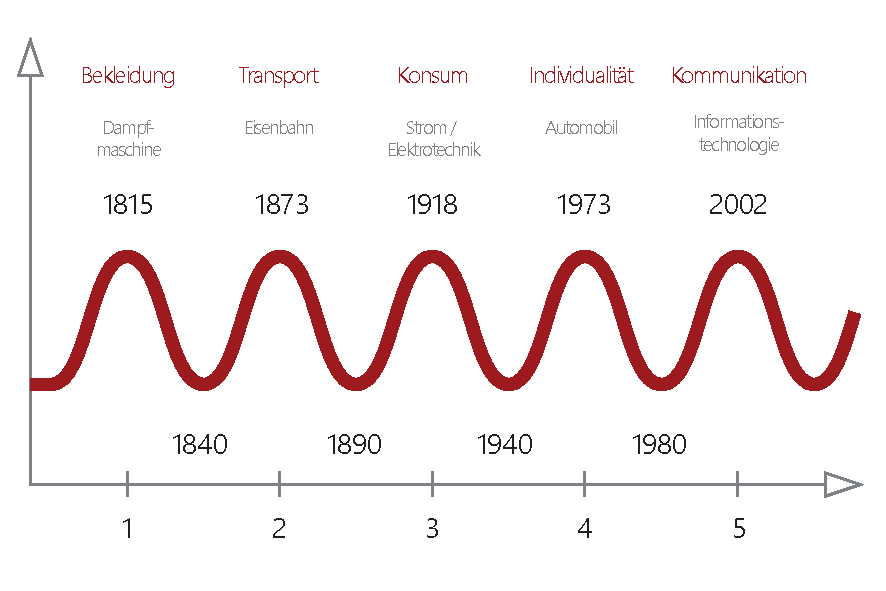
\includegraphics[angle=0,width=12cm]{./img/zyklen.pdf}}
  \caption{Kondratieff-Zyklen}
  \label{zyklen}
  \vspace{0.5cm}
\end{figure}

Diese Erfindung gilt als Beginn des ersten Kondratieff-Zyklus. Vor dem maschinellen Betrieb wurden Spinnräder noch manuell bedient und Kleidung war teuer. Die dampfbetriebenen Webstühle steigerten
die Effizienz um das 200-fache. In den 20er Jahren stagnierte die Branche, da die Rohstoffbeschaffung und Warenverteilung das Maximum der Effizienz erreicht hatte. Mit der Erfindung der Eisenbahn gelang der Übergang vom ersten in den zweiten Zyklus. In den folgenden Jahren konnte nun das Bedürfnis nach verbesserten Transportmöglichkeiten gestillt werden.\\
Dampfmaschine, Eisenbahn, Strom, Motor und der Mikrochip stehen alle für eine Basisinnovation, die zukünftige Gesellschaften geprägt haben. Im lauf der Zeit verschwinden die Erfindungen aus dem Bewusstsein der Menschen und werden zu Gegenständen des Alltags. Motor und Mikrochip sind so stark im gesellschaftlichen Leben verankert, dass sie nicht mehr direkt wahrgenommen werden. Betrachtet man eine elektrische Zahnbürste, ist es selbstverständlich, dass die Energie aus dem Stromnetz bezogen wird und der Bürstenkopf von einem Motor angetrieben wird.\\
Das Jahr 2002 gilt als Höhepunkt des fünften Kondratieff-Zyklus und die Gesellschaft befindet sich gerade im Übergang zum Sechsten. Noch fehlt die aktuelle Basisinnovation und auch das zu stillende Bedürfnis ist nach der Kommunikation noch nicht bestimmt.\\
Nach Nefiodow \cite{nefiodow:gesundheit} gibt es vier Möglichkeiten welcher Markt in Zukunft den sechsten Kondratieff prägen wird:
\begin{itemize}
  \item \textbf{Informationsmarkt} \\
  		Mobile Geräte und Soziale Netzwerke sind maßgebend für diesen Markt. So verhalf der Kurznachrichtendienst Twitter zum sogenannten \glqq Arabischen Frühling\grqq\, durch die blitzschnelle Kommunikation über das Netz\footnote{http://www.heise.de/tr/blog/artikel/Wie-funktioniert-die-Twitter-Revolution-1761481.html \\aufgerufen am 06.01.2014}.
  \item \textbf{Bio - und Nanotechnologie} \\
  		Die Erfindung des Mikroskops und die Entschlüsselung der DNA im Jahr 2000 gilt als Basisinnovation. Anfangs wurden die Erkenntnisse nur in Medizin und Pharmazie angewendet. Heute profitiert auch die Landwirtschaft und Lebensmittelindustrie davon.
  \item \textbf{Umwelttechnologie}
  		Auch der Bereich Umwelttechnologie sorgte für einen Zuwachs an Arbeitsplätzen. In Deutschland standen im Bereich der erneuerbaren Energien 170.000 Menschen in einem Beschäftigungsverhältnis\footnote{vgl. \cite{nefiodow:gesundheit} S. 107}.
  \item \textbf{Gesundheit}
  		Der Gesundheitsmarkt vereint technologische Komponenten wie die Medizintechnik und psychosoziale Gesundheit. Es erfolgt ein Wechsel vom heutigen \glqq Krankheitswesen\grqq\ zum Gesundheitswesen, angefangen von der Burnout-Prophylaxe, Gesundheitstourismus zur Bionik und künstlichen computergesteuerten Prothesen.
\end{itemize}

\section{Wachstumsmarkt Gesundheit}

Nach Granig\cite{nefiodow:gesundheit} ist der Gesundheitsbereich der derzeit am schnellsten wachsende Markt\footnote{Gemessen am Anteil der Branche am Bruttoinlandsprodukt}. Die Bevölkerung ist gewillt in die eigene Gesundheit zu investieren und die Unternehmen positionieren sich im Gesundheitsbereich (Siemens beispielweise verstärkt sich im Bereich der Medizintechnik).
Die Bio- und Nanotechnologie und die Medizintechnik ähneln sich in einigen Bereichen. Sowohl Siemon Cord \cite{cord:innovation} als auch Granig\footnote{vgl. \cite[Seite 116 f]{nefiodow:gesundheit} } sprechen davon, dass der Markt sich nur gehemmt entwickeln kann. Grund dafür sind sowohl in der Nano- als auch Medizintechnik veraltete Gesetzte und auch ethnische Hürden, die es zu überwinden gilt.\\
Cord schreibt, dass 100\% des Wissens der Biotechnik aus Hochschulwissen stammt (allerdings aufgrund der erwähnten Einschränkungen noch nicht ökonomisch verwertet werden kann). Zwar trifft diese hohe Prozentzahl nicht auf die Medizintechnik zu, da viel Entwicklung in den Unternehmen stattfindet, doch der Grundstein für Innovation wird bei den Studierenden der Hochschulen und Universitäten gelegt. Die Bildungseinrichtungen werden ein zentrales Standbein für den kommenden sechsten Kondratieff mit einem Schwerpunkt Bio-, Medizintechnik und Gesundheit sein.

\section{Der Studiengang Biomedizinische Technik}\label{einleitung:biomedTechnik}
In einem Onlineartikel vom Februar 2012\footnote{https://www.haw-landshut.de/aktuelles/news/news-archiv/news-detailansicht/article/neuer-studiengang-biomedizinische-technik-vielfaeltige-berufschancen.html \\ abgerufen am 10.01.2014} veröffentlichte die Hochschule Landshut, dass ab dem Wintersemester 2012 der neue Bachelorstudiengang \glqq Biomedizinische Technik\grqq\ angeboten wird. Auch der Artikel beschreibt, ähnlich wie Granig, die Medizintechnik als Wachstumsmarkt und bestätigt, auch durch die Einführung des Studiengangs, das gesellschaftlich gesteigerte Interesse am Gesundheitswesen.\\
Während des Studienverlaufs \cite{hsla:modulBMT} erwerben die Studierenden vor allem im zweiten Studienabschnitt Kenntnisse im Bereich der Medizintechnik. Die Ausbildung behandelt unter Anderem bildgebenden Systeme, medizinische Bildverarbeitung und minimalinvasive Therapieverfahren.\\
Für die Ausbildung stehen Labore mit den benötigten Geräten zur Verfügung, um mit dem theoretischen Wissen praktisch zu experimentieren.

\section{Das Labor für medizinische Bildverarbeitung, Algorithmen und Krankenhaus IT}\label{einleitung:labor}
Das Labor erfüllt zwei Interessen. Die Ausstattung steht für die Forschung, interessierten Unternehmen und Krankenhäusern zu Verfügung.
Für die Lehre soll Studierenden die Möglichkeit geboten werden, den Prozess der medizinischen Bildverarbeitung anschaulich und praxisnah zu erleben. Mittels Doppler-Ultraschallgerät können Bilddaten erzeugt und anschließend an das Picture Archiving and Communication System\footnote{Ein PACS dient als zentraler Bildspeicher, der über das Netzwerk angesprochen werden kann. Medizinische Geräte legen dort die Bilddaten ab, während die Software zu Betrachtung die Daten vom PACS holt} (PACS) gesendet werden. Anschließend können Algorithmen zur Bildvorverarbeitung, Merkmalsextraktion oder auch Segmentierung implementiert und getestet werden.\\
Medizinische Bilddaten unterscheiden sich maßgeblich von allgemeinen Bildformaten wie JPEG oder Bitmaps, daher sind zur Betrachtung sogenannte DICOM-Viewer\footnote{DICOM (Digital Imaging and Communications in Medicine) ist der heutige Standard der medizinischen Informationsverarbeitung und wird in den folgenden Kapiteln näher erläutert. Die Viewer ermöglichen die Betrachtung der Bilddaten} notwendig. Mit Hilfe dieser Programme lassen sich die erzeugten Bilder betrachten und grundlegende Operationen auf diesen anwenden (dazu zählt beispielsweise die Skalierung oder Verschiebung des Bildes). Komplexe Bildverarbeitungsalgorithmen können allerdings nicht ausgeführt oder selbst implementiert werden.\\
Für Forschung und Lehre wird eine Software benötigt, die sowohl die Grundfunktionen der Betrachtung liefert, als auch eine Schnittstelle zur eigenen Erweiterung zu Verfügung stellt.



\chapter{Grundlagen medizinischer Daten- und Bildformate} \label{grundlagen}
\addthumb{Grundlagen der medizinischen Bildverarbeitung}{\huge{\textbf{\thechapter.}}}{white}{haw_rot}

\section{Bildgewinnung und bildgebende Verfahren}\label{grundlagen:bildgebung}

\section{DICOM}\label{grundlagen:dicom}
Der Name DICOM steht für \textit{Digital Imaging and COmmunication in Medicine}. Der Umgang mit diesem Standard ist essentieller Bestandteil der zu entwickelnden Software. Pianykh\cite{pianykh:dicom} beschreibt im ersten Kapitel, dass DICOM nicht nur aus Pixel und deren zugehörigen Werten besteht. Wie der Name sagt, ist auch die Kommunikation fest im Standard verankert. Damit ist die Übertragung der Daten von medizinischen Geräten(Modalitäten) zum zentralen Speicher und deren Verteilung gemeint. Des weiteren spielt die dauerhafte Speicherung der digitalen Aufnahmen eine große Rolle. Daher wird im gleichen Zug mit DICOM immer ein PACS genannt. Das Akronym PACS bedeutet \textit{Picture Archiving and Communication System} und besteht sowohl aus Hardware (Server, Speicherung) als auch Software(Verteilung und Kommunikation).\\
Abbildung \ref{communication} illustriert das Zusammenspiel des DICOM-Standards und dem zentralen Datenspeicher. Zuerst wird mittels der Modalitäten(z.B. mit dem Computertomographen oder einem Ultraschallgerät) die digitale Aufnahme erzeugt. Danach wird das Bild vom Gerät an das PACS gesendet. Hier werden die Aufnahmen und Patientendetails in die Datenbank und den Speicher abgelegt. Wird eine Aufnahme benötigt können Clients Anfragen mit beispielsweise dem Patientennamen stellen und erhalten die zugehörige Serie mit der digitalen Aufnahme.

\begin{figure}[htbp]
  \vspace{0.5cm}
  \centering
  \fbox{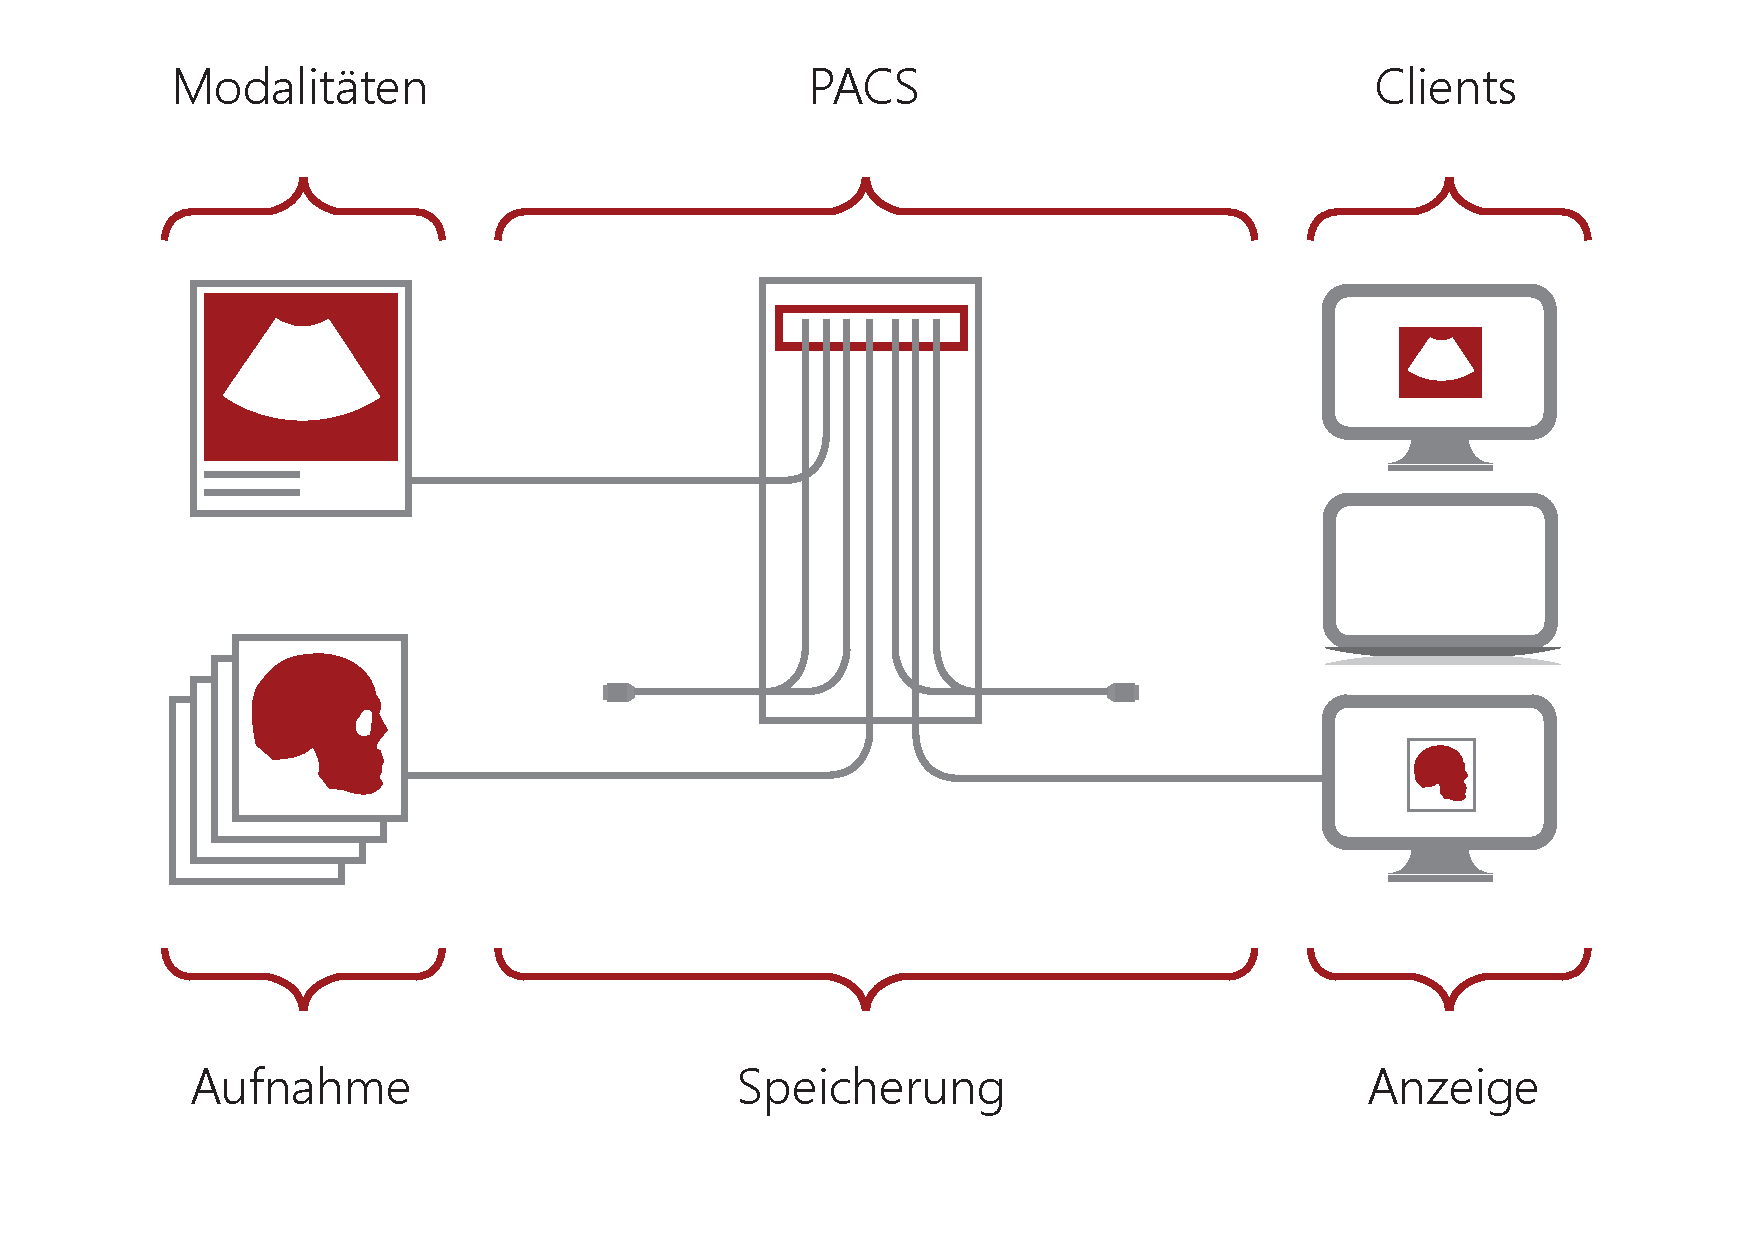
\includegraphics[angle=0,width=12cm]{./img/communication_neu.pdf}}
  \caption{Kommunikationsprozess von Aufnahme zur Verarbeitung}
  \floatfoot{Vorlage für diese Darstellung ist die Grafik in \cite[Fig. 1]{pianykh:dicom}}
  \label{communication}
  \vspace{0.5cm}
\end{figure}

DICOM\footnote{Unter ftp://medical.nema.org/medical/dicom/ lässt sich der aktuelle Standard abrufen. Die Kapitel befinden sich im Ordner zum jeweiligen Jahr der Veröffentlichung. Aktuell sind die Dokumente von 2011.} ist daher nicht nur ein einzelner Standard, sondern verknüpft die standardisierte 
\begin{itemize}
\item Kommunikation,
\item Erzeugung der Bilddaten,
\item und Speicherung.
\end{itemize}
Im Rahmen dieser Abschlussarbeit liegt der Fokus auf den Bilddaten, daher wird auf die Kommunikation- und Speicheraspekte nicht im Detail eingegangen.

\subsection{Die Dicom Information Object Definitionen} \label{grundlagen:iod}
Bevor die Pixeldaten genauer betrachtet werden können, muss der prinzipielle Aufbau der Dicomobjekte beschrieben werden. Teil 3 des Standards\cite[A.1.2]{dicom:iod} zeigt den relationalen Aufbau der Dicomobjekte. Vereinfacht können die elementaren Informationsobjekte in drei Teile aufgeteilt werden.

\begin{itemize}
	\item \textbf{Patient}\\
	Der Patient steht in der Hierarchie an oberster Stelle und ist die Grundlage für eine oder mehrere Studien(Study).
	\item	\textbf{Study}\\
	Study symbolisiert eine medizinische Studie. Eine Studie ist eine Sammlung von mehreren Serien, die von Modalitäten wie CT und MR aufgezeichnet werden. Eine Studie ist exakt einem Patient zugeordnet.
	\item \textbf{Series}\\
	Eine Serie ist ein Folge von Bildern, die von einer Modalität erzeugt wird. Die Aufnahmen eines CT werden einer Serie zugeordnet. Jede Serie gehört zu nur einer Studie.
	\item \textbf{Image, Real World Values}\\
	Auf der unteren Hierarchiestufe stehen Objekte wie Bilddaten oder die Lage des Patienten im Raum während der Aufnahme. Ein Bild wird genau einer Serie zugeordnet.
\end{itemize}

Aus diesen vier elementaren Objekten ergibt sich folgende Informationsstruktur für Dicomobjekte, die in Abbildung \ref{ermodel} als Entity-Relationship-Modell\footnote{Ein ER-Modell beschreibt die Beziehungen der Elemente zueinander. Dieser Diagrammtyp wird unter Anderem häufig beim Entwickeln der Struktur einer relationalen Datenbank verwendet} verdeutlicht wird.

\begin{figure}[htbp]
  \vspace{0.5cm}
  \centering
  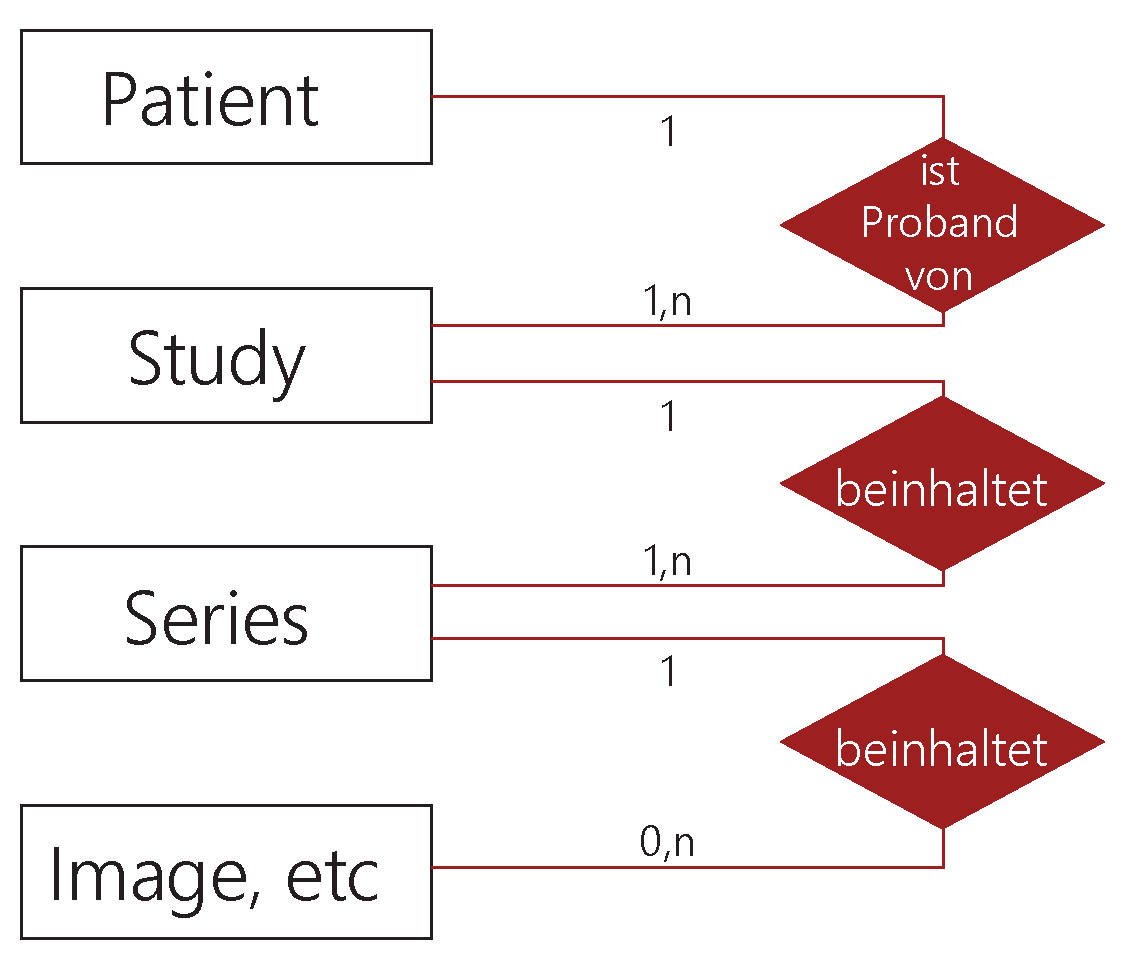
\includegraphics[angle=0,width=8cm]{./img/ermodel.pdf}
  \floatfoot{Vorlage für diese Darstellung ist die Grafik in \cite[A.1.2]{dicom:iod}}
  \caption{Vereinfachte Darstellung der Informationsobjekthierarchie von Dicomelementen}
  \label{ermodel}
  \vspace{0.5cm}
\end{figure}

Der DICOM-Viewer OsiriX bietet auf der Herstellerseite\footnote{http://www.osirix-viewer.com/datasets/} die Möglichkeit Testdaten zu beziehen. Betrachtet man die Repräsentation der Daten auf der Festplatte hält sich die Ordnerstruktur an obiges ER-Modell.\\
Abbildung \ref{filesystemrep} zeigt eine schematische Darstellung der Dateien. Die Beispieldaten von OsiriX bestehen aus einem Patient names \glqq Brebix\grqq\, dem eine Studie sowie zwei Serien à 100 Aufnahmen zugeordnet werden.

\tikzstyle{every node}=[draw=black,thick,anchor=west]
%\tikzstyle{selected}=[draw=red,fill=red!30]
\tikzstyle{optional}=[dashed,fill=gray!50]
\begin{figure}[htbp]
\centering
\caption{Repräsentation der Information Objekte im Dateisystem}
\label{filesystemrep}
\begin{tikzpicture}[%
  grow via three points={one child at (0.5,-0.7) and
  two children at (0.5,-0.7) and (0.5,-1.4)},
  edge from parent path={(\tikzparentnode.south) |- (\tikzchildnode.west)}]
  \node {Dicom Ordner}
    child [missing] {}
    child { node {BREBIX - Patient}
    	child [missing] {}
    	child { node{CT10 ponction foie - Studie}
    		child [missing] {}
    		child { node {DEF FOIE ART. - 107198 - Serie}
    			child{node[optional]{IM-0001-0001.dcm}}
    			child{node[optional]{...}}
    			child{node[optional]{IM-0001-0100.dcm}}
    		}
    		child [missing] {}				
    		child [missing] {}				
    		child [missing] {}
    		child [missing] {}
    		child { node {DEF. VEINEUX - 107205 - Serie}
    		    child{node[optional]{IM-0001-0001.dcm}}
    		    child{node[optional]{...}}
    		    child{node[optional]{IM-0001-0100.dcm}}
    		}
    		child [missing] {}
    	}
    };		
\end{tikzpicture}
\end{figure}

Bei näherem Hinsehen fällt auf, dass die Dateinamen beider Serien des Patienten identisch sind. Eine korrekte Zuordnung von DICOM-Dateien zur Serie ist daher nicht immer garantiert. Unabhängig von einer Repräsentation im Dateisystem oder Pfadangaben in der Datenbank eines PACS ist das Vertrauen auf Dateipfade unsicher, da über eine einfache Dateimanipulation die Zuordnung nicht mehr hergestellt werden kann.\\
Um eine zuverlässige Verknüpfung zu gewährleisten besitzt jeder Patient\footnote{Die Identifikationsnummern von Patienten sind meist nur innerhalb einer Institution oder Krankenhauses einzigartig, da diese manuell vergeben werden können\cite[5.6.2]{pianykh:dicom}.}, jede Studie und jede Serie eine Eindeutige Identifikationsnummer. Diese Art der Informationen wird in den einzelnen Dateien mit Hilfe von Einträgen aus dem DICOM Data Dictionary\cite{dicom:dd} hinterlegt. Die DICOM-Dateien beschreibt Pianykh \cite[S. 47]{pianykh:dicom}
als eine Kopie im Speicher vom tatsächlichen DICOM-Objekt.

\subsection{Der Transfer vom Patienten zu digitalen Dicomobjekten} \label{grundlagen:dicomObjects}
Wie der Name bereits andeutet ist das DICOM Data Dictionary vergleichbar mit einem Wörterbuch. Es enthält alle gültigen Elemente, die zur Beschreibung eines DICOM-Objekts verwendet werden können. Zusätzlich zu dem aus dem Standard bekannten Vokabular können Hersteller medizinischer Geräte ein eigenes Dictionary hinzufügen. Die proprietären Elemente können allerdings nicht standardisiert verarbeitet werden(vgl. \cite[S.45]{pianykh:dicom}, da Software die diese Objekte verarbeitet, nichts von der Existenz dieser Elemente weiß).\\
Mit Hilfe des Wörterbuchs und den ca. 2000 enthaltenen Daten können nun Aussagen des wirklichen Lebens (vorausgesetzt die Aussage ist mit einem Element aus dem Wörterbuch darstellbar) ins Digital übersetzt werden.\\
Tabelle \ref{table:patientname} zeigt das DICOM-Element für den Namen des Patienten aus dem Data Dictionary\cite[S. 14]{dicom:dd}.

\begin{table}
    \begin{tabularx}{\textwidth}{|X|X|X|X|X|}
    \toprule
    \hline
    \textbf{Tag}         & \textbf{Tagname}     & \textbf{VR} & \textbf{Wert}     	& \textbf{VM} \\ \hline
    (0010,0010) 		 & PatientName 			& PN 		  & John\^{}Doe 		& 1  \\  \hline
    \bottomrule
    \end{tabularx}
    \caption {Repräsentation des Patientennamen als DICOM-Element}
    \label{table:patientname}
\end{table}

Betrachtet man den folgenden Satz(vgl. \cite[S.46]{pianykh:dicom}), kann dieser in ein DICOM-Object, wie es Tabelle \ref*{table:translation} darstellt, übersetzt werden:
\begin{center}
\textit{\glqq John Doe, männlich, geboren am 01. Januar 1970\grqq}
\end{center}

Aus den Beispielen von Tabelle \ref{table:patientname} und \ref{table:translation} lässt sich erkennen, dass ein DICOM-Element nochmals in atomare Teile aufgespalten werden kann. Folglich besteht ein Datenelement aus einem beschreibenden \textit{Tag}, einer \textit{VR(Value Representation)}, einem Wert und der \textit{VR (Value Multiplicity)}. Das Element selbst nimmt eine von drei Darstellungsmöglichkeiten ein. Zusätzlich liegt im Speicherabbild des Datenelements die Länge des Wertes\footnote{John\^{}Doe besitzt aufgrund der Zeichenmenge eine Länge von acht}. Abhängig von der Transfersytax\footnote{Unter der Transfersystax verstehn man eine Menge an Kodierungsvorschriften von DICOM-Objekten\cite[S.63 Section 10]{dicom:structure}. Zu diesen Vorschriften gehört zum Beispiel die Reihenfolge der Bytes im DICOM-Element oder die Komprimierung der Bilddaten} des DICOM-Objekts ist der VR-Teil optional. Die weiteren beiden Darstellungen unterscheiden sich in der Kodierung der benötigten Länge des Werts \cite[7.1]{dicom:structure}.  Anhang \ref{appendix:speicher} auf Seite \pageref{appendix:speicher} zeigt wie Datenelemente im Speicher abgelegt werden und wie viel Speicherplatz pro Element reserviert werden muss.

\begin{table}
    \begin{tabularx}{\textwidth}{|p{4cm}|p{4cm}|X|X|X|}
    \toprule
    \hline
    \textbf{Tag\newline \small{(Gruppe, Element)}}         & \textbf{Tagname}     & \textbf{VR} & \textbf{Wert}     	& \textbf{VM} \\ \hline
    (0010,0010) 		 & PatientName 			& PN 		  & John\^{}Doe 		& 1  \\ \hline
    (0010,0030) 		 & PatientBirthDate		& DA 		  & 19700101	 		& 1  \\ \hline
    (0010,0040)			 & PatientSex 			& CS 		  & M			 		& 1  \\ \hline
    (0010,1010) 		 & PatientAge 			& AS 		  & 44			 		& 1  \\ \hline
    \bottomrule
    \end{tabularx}
    \caption {Das erzeugte DICOM-Objekt mit den Elementen zu Patientenname, Geburtsdatum, Geschlecht und Alter}
    \label{table:translation}
\end{table}

\subsection{Tags in Datenelementen}

Ein DICOM-Element wie PatientName kann über ein Tag identifiziert werden. Ein Tag ist in einem DICOM-Objekt einzigartig und darf nur ein mal benutzt werden. Die numerische Darstellung hat die Form (\textit{gggg}, \textit{eeee}) wobei die hexadezimalen Ziffern \textit{g} die Gruppe des DICOM-Elements beschreiben und \textit{e} das Element der Gruppe \textit{g} definiert. Zusätzlich zu diesen Eigenschaften, kann bestimmt werden, ob der Ursprung eines DICOM-Elements im Standard- oder einem privaten Data Dictionary liegt. Eine gerade Gruppen-Ziffer zeigt, dass das Element Teil des Standards ist während ungerade für proprietäre Elemente stehen\footnote{Ausgenommen aus dieser Regel sind folgende Gruppen: (0000, eeee), (0002, eeee), (0004, eeee), (0006, eeee), (0001, eeee), (0003, eeee), (0005, eeee), (0007, eeee), (FFFF, eeee)}\cite[7.1]{dicom:structure}. Die Reihenfolge der Tags ist in numerischer Folge in aufsteigender Form sortiert. Fällt während des Einleseprozesses in eine Datei auf, dass die Reihenfolge nicht korrekt ist, deutet dies auf ein korruptes DICOM-Objekt hin.\\

\subsection{VR - Value Representation}
Dieser Teil eines DICOM-Elements beschreibt den Typ und das Format des Wertes\cite[6.2]{dicom:structure}. Der Umfang an verschiedenen Value Representations reicht von Zeichenketten wie PersonName (PN) im Datenelement (0010,0010) PatientName über Datumsangaben (DA) bis zu numerischen Werten(FL) und Sequenzen (SQ). Eine vollständige Liste ist im Standard unter \cite[Table 6.2.1]{dicom:structure} zu finden.\\
Zwecks Vollständigkeit soll erwähnt werden, dass ein Datenelement mit VR-Typ SQ wiederum ein DICOM-Object enthalten kann und dadurch eine Baumstruktur entsteht.

\subsection{VM - Value Multiplicity}
Value Multiplicity bestimmt die Anzahl an Werten, die in einem DICOM-Element enthalten sind. Die Werte werden durch einen Backslash \textbackslash voneinander getrennt. Der explizite Wert der Value Multiplicity kann aus dem Data Dictionary entnommen werden.\cite[6.4]{dicom:structure}

\section{DICOM Pixeldaten und Bildformate}

Die Abschnitte \ref{grundlagen} - \ref{grundlagen:dicomObjects} zeigen, dass DICOM mehr als ein Bildformat darstellt, ein essentieller Bestandteil bleiben jedoch die Pixel eines DICOM-Objekts (auch wenn diese nur optional vorhanden sein müssen, wie Grafik \ref{ermodel} zeigt). Nach dem DICOM Data Dictionary gehören Bild-abhängige Informationen zur Gruppe (\textit{0028}, \textit{eeee}).
Die Pixeldaten liegen im Bereich (\textit{7fe0}, \textit{0010}) am Ende eines DICOM-Objekts.\\
Das bedeutet, dass die konkreten Werte der Pixel im gleichen DICOM-Objekt liegen und den selben Kodierungsrichtlinien der DICOM-Tags unterliegen.

\subsection{Kodierung der Pixel im Speicherabbild eine DICOM-Objekts} \label{pixelkodierung}

Um die grundlegende Struktur der Pixel im DICOM-Objekt zu beschreiben sind drei Datenelemente notwendig: BitsAllocated, BitsStored und HighBit\ref{table:digitalRep}. BitsAllocated beschreibt, wie viel Speicher für einen singulären Pixelwert reserviert wird. Mit Hilfe von Columns und Rows kann die Bilddimension bestimmt werden. Columns beschreibt die Breite, Rows die Höhe. Die Value Representation des Datenelements PixelData (\textit{7fe0}, \textit{0010}) kann nach DICOM Data Dictionary entweder den Wert \textit{OB} oder \textit{OW} annehmen. OB bedeutet \textit{Other Byte String} während OW für \textit{Other Word String} steht. Nach Section 8.1 des Standards\cite{dicom:structure} besteht der Unterschied zwischen den beiden VRs darin, dass OB abhängig von der Byteordnung ist. Ob die Ordnung Little Endian oder Big Endian entspricht ist abhängig von der Transfersyntax des DICOM-Objekts.
Grafik \ref{byteorder} zeigt die Kodierungsreihenfolge. Little Endian kodiert vom Least Significant Bit (LSB) zum Most Significant Bit (MSB). Big Endian verarbeitet die Byte in umgekehrter Reihenfolge. Ein Element von PixelData (sowohl mit einer VR von OB als auch OW) fasst 16 Bit, was gleichzeitig die maximale Größe an allokiertem Speicher von BitsAllocated darstellt.

\begin{figure}[htbp]
  \vspace{0.5cm}
  \centering
  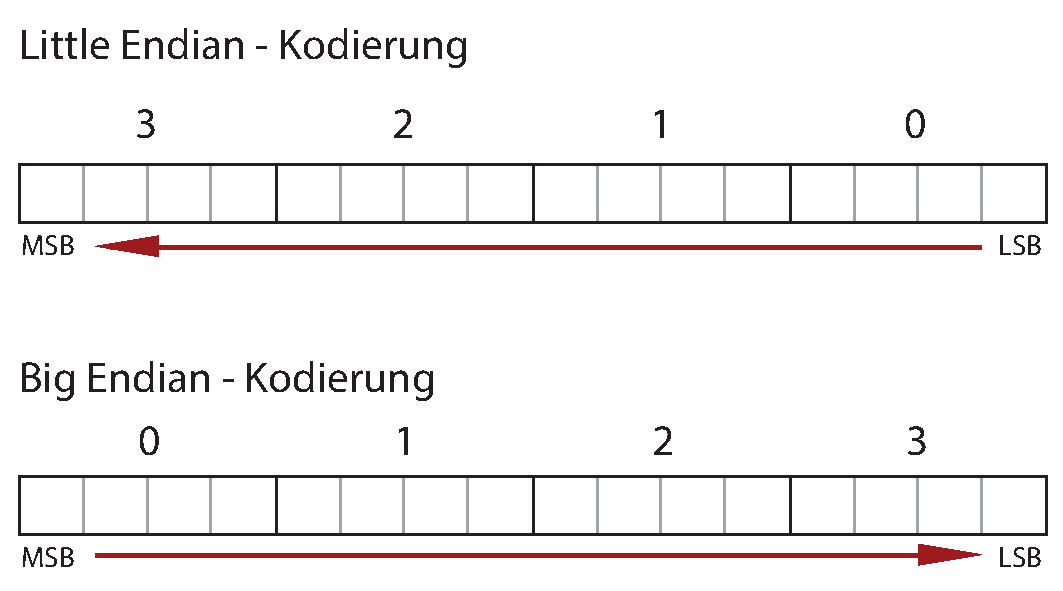
\includegraphics[angle=0,width=10cm]{./img/byteorder.pdf}
  %\floatfoot{Vorlage für diese Darstellung ist die Grafik in \cite[A.1.2]{dicom:iod}}
  \caption{Kodierungsreihenfolge von 4 Byte bei Little Endian- und Big Endian-Darstellung}
  \label{byteorder}
  \vspace{0.5cm}
\end{figure}

BitsStored gibt darüber Auskunft, wie viel Bit pro Wert in Anspruch genommen werden. Schließlich gibt HighBit das in der Reihenfolge ranghöchste Bit von StoredBits an \cite[8.1.1]{dicom:structure}.\\
Abbildung \ref{bits:pixel} verdeutlicht die Repräsentation eines Pixels im Datenelement PixelData. Die Darstellung entspricht einem eindimensionalen Array. Das erste Element ist das erste Pixel in der linken oberen Ecke, das letzte Element stellt den Pixel rechts unten dar. \ref{bits:16} und \ref{bits:8} zeigen die exakte Belegung an Bit bei BitsStored 16 und BitsStored 8. Der graue Hintergrund zeigt die allokierten Bit, während der rote Bereich den tatsächlich benutzten Speicher markiert. Der Pixelwert in Abbildung \ref{bits:8} nimmt den gesamten Speicherplatz pro Pixel ein. Das schwarze Quadrat steht für das HighBit.\\
Das Intervall der Werte ist abhängig von der Anzahl an gespeicherten Bits. Hat das Element StoredBits den Wert 12 kann ein  Pixel einen Wert aus dem Bereich von $[0, 2^{12}-1]$ annehmen. Entspricht StoredBits 8 ist das Intervall $[0, 2^8-1]$. Hier spricht man von einer Grauwerttiefe von 12 beziehungsweise 8 \cite[2.2]{handels:mbv}.
\begin{figure*}[htb]
%\subfigure[Keypoints]{\includegraphics[width=0.49\textwidth]{./img/basmati_keypoints.png}}\hfill
\centering
\fbox{
\subfigure[Pixel im Speicher]{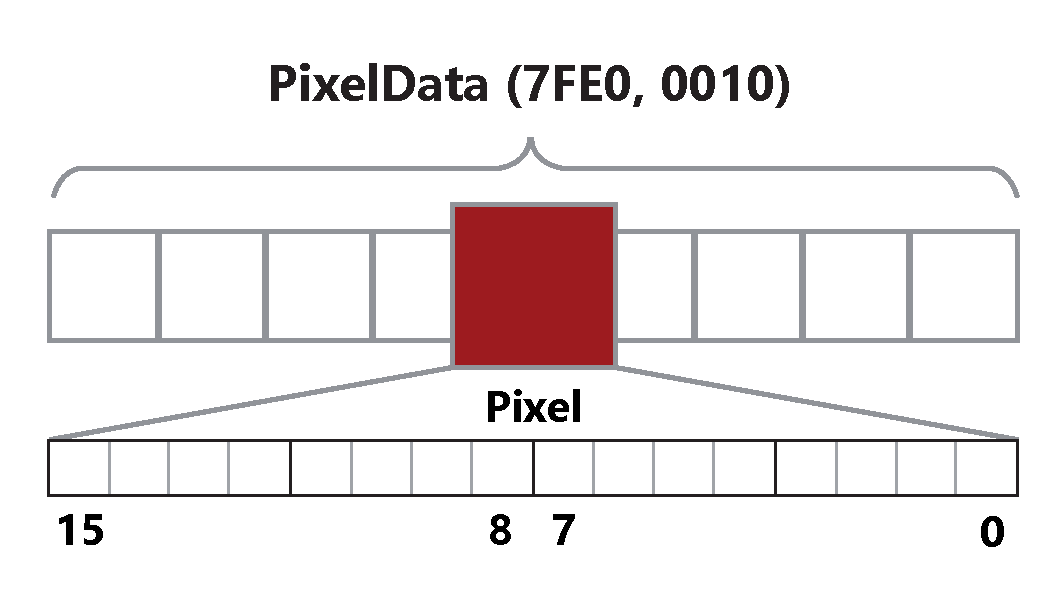
\includegraphics[width=5cm]{./img/bits.pdf} \label{bits:pixel}}
\subfigure[BitsAllocated 16, BitsStored 12, HighBit 11]{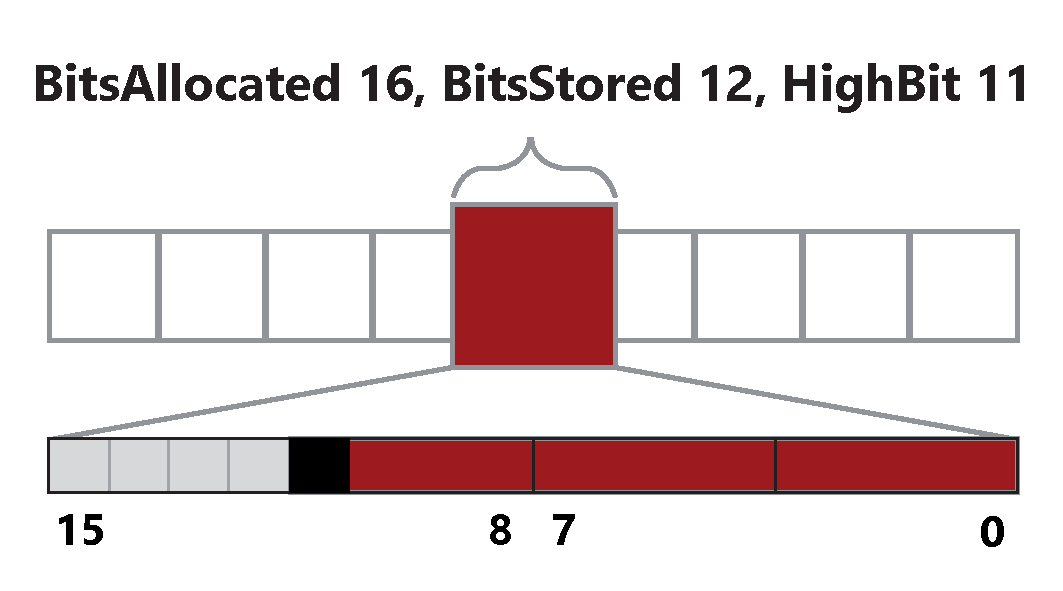
\includegraphics[width=5cm]{./img/bits16.pdf} \label{bits:16}}
\subfigure[BitsAllocated 8, BitsStored 8, HighBit 7]{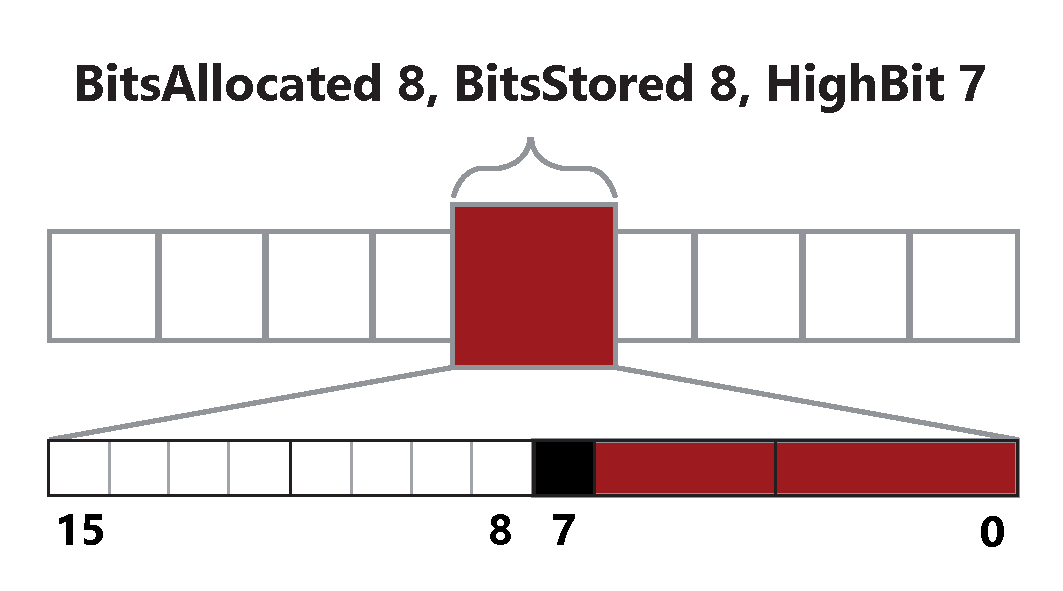
\includegraphics[width=5cm]{./img/bits8.pdf} \label{bits:8}}
}
\caption{Beispiele unterschiedlicher Speicherbelegung}
\label{bits}
\end{figure*}

Verschiedene Datenelemente aus dem DICOM-Standard liefern nähere Informationen zum Bildformat. So gibt das Element SamplesPerPixel (0028,0002) Auskunft darüber, wieviel Teile aus PixelData ein einzelnes Pixel repräsentieren. Hat Samples den Wert 1, so ist jedes Element aus PixelData genau ein Pixel. Daraus folgt, dass ein Grauwertbild vorliegt. 3 bedeutet, dass im DICOM-Objekt ein Farbbild mit den drei Kanälen rot, grün und blau liegt.\\
Die Werte der Pixel sind stark abhängig vom medizinischen Gerät, welches die Bilder aufzeichnet. Ein direkter Vergleich von Bildern, die von unterschiedlichen Geräten einer Modalität aufgezeichnet wurden ist daher nicht möglich. Um Gewebestrukturen von beispielsweise CT-Aufnahmen trotz dieser Abhängigkeiten patienten- und geräteübergreifend zu vergleichen, gibt es unter Anderem die Hounsfield Skala \cite[2.1.3]{handels:mbv}. Mit Hilfe der Datenelemente RescaleSlope und RescaleIntercept lassen sich die ursprünglichen Werte in brauch- und lesbare Pixelwerte konvertieren. RescaleType gibt die Skala an, mit der das Ergebnis interpretiert werden kann. Ein Umrechnung erfolgt mit der Formel aus \cite[C.11-1b Seite 1168]{dicom:iod}\\

\begin{equation}
Output=m*SV+b
\label{rescale}
\end{equation}

mit $m = RescaleSlope$, $b = RescaleIntercept$ und $SV=Pixelwert$.

Fettgewebe zum Beispiel nimmt nach der Hounsfield-Skala Werte zwischen 0 und -100 ein \cite[Abbildung 1.18 Seite 15]{radio:hounsfield}. Ob in einem DICOM-Objekt vorzeichenbehaftete Werte vorhanden sind, sagt das Element PixelRepresentation. Eine 0 bedeutet kein Vorzeichen. Bei einem Wert von 1 können negative Werte enthalten sein.
\begin{table}
    \begin{tabularx}{\textwidth}{|X|X|X|}
    \toprule
    \hline
    \textbf{Tag}         & \textbf{Tagname}     & \textbf{VR} \\ \hline
    (0028,0010) 		 & Rows					& US 		  \\ \hline
    (0028,0011) 		 & Columns				& US 		  \\ \hline
    (0028,0100) 		 & BitsAllocated		& US 		  \\ \hline
    (0028,0101) 		 & BitsStored			& US 		  \\ \hline
    (0028,0102)			 & HighBit				& US 		  \\ \hline
    \bottomrule
    \end{tabularx}
    \caption {Grundlegende Datenelemende für die digitale Repräsentation}
    \label{table:digitalRep}
\end{table}

\subsection{Grauwertbilder} \label{grey_images}

Für Bildverarbeitungsprozesse und Algorithmen bieten Grauwertbilder einige Vorteile im Vergleich zu Farbbildern. Der größte Unterschied liegt beim Verhältnis zwischen Informationsgehalt zu Speicherbedarf. Farben bieten bei Kantenübergängen oder Helligkeitsinformationen keinen Mehrwert. Das führt unter Anderem dazu, dass Industrie oder auch die medizinische Bildverarbeitung vorwiegend auf dieses Format zurückgreifen.\\
Eine Grauwerttiefe von 8 Bit ist Standard in der Bildverarbeitung. Das entspricht dem Intervall von $[0,255]$ und den Werten, die mit handelsüblichen Monitoren darstellbar sind. Medizinische Bilddaten können, wie in Abschnitt \ref{pixelkodierung} beschrieben, eine Tiefe von bis zu 16 Bit annehmen und Grauwerte aus dem Bereich $[0,65535]$ repräsentieren.

\begin{figure*}[htb]
%\subfigure[Keypoints]{\includegraphics[width=0.49\textwidth]{./img/basmati_keypoints.png}}\hfill
\centering
\fbox{
\subfigure[CT]{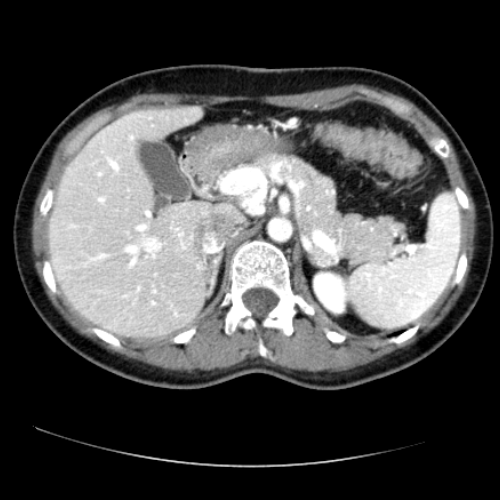
\includegraphics[width=5cm]{./img/ct.png} \label{ct}}
\subfigure[MR]{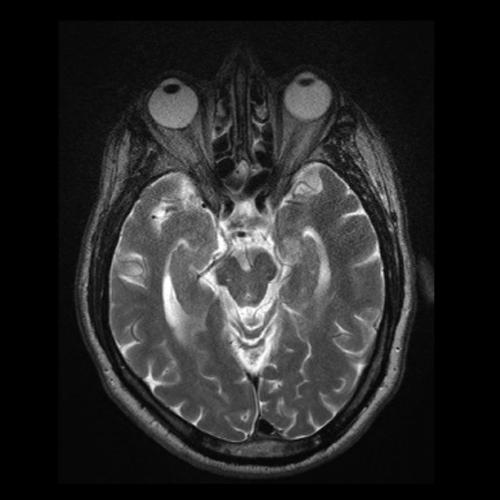
\includegraphics[width=5cm]{./img/mr.png} \label{mr}}
\subfigure[Ultraschall]{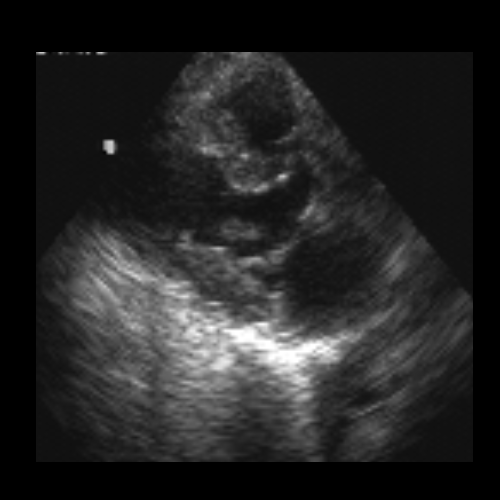
\includegraphics[width=5cm]{./img/sono.png} \label{sono}}
}
\floatfoot{Die Beispieldaten stammen von http://www.osirix-viewer.com/datasets/ - abgerufen am 19.01.2014}
\caption{Verschieden Graustufenbilder}
\label{grey}
\end{figure*}

\subsubsection{Fensterung von Grauwerten} \label{windowing}

Wie bereits in \ref{grey_images} beschrieben, lassen sich auf üblichen Monitoren nicht alle Grauwerte zur gleichen Zeit anzeigen. Dadurch müssen die maximal 65535 verschiedenen Grauwerte auf 255 abgebildet werden können. Dies wird durch die in der Radiologie verwendete Fensterungstechnik möglich\cite[Kapitel 8, Seite 249]{handels:mbv}. Es wird ein Fensterzentrum und eine Fensterbreite gewählt. Alle Werte innerhalb dieses Intervalls werden zwischen 0 und 255 umgerechnet. Abbildung \ref{window_graph} verdeutlicht dieses Prinzip. Ein CT-Bild mit einer Tiefe von 12 Bit besitzt 4096 Grauwerte. Ein Zentrum von 2000 und eine Breite von 500 bildet alle Werte von 1750 bis 2250 auf 0 bis 255 ab. Ist ein Pixeldatum kleiner 1750 wird das Minimum 0 hinterlegt und ist der Wert größer 2250 bekommt das Pixel das Maximum 255.\\
Im DICOM-Standard ist ein Algorithmus gegeben, um die Pixeldaten zu konvertieren\cite[C.11.2.1.2]{dicom:iod}.

\begin{algorithm}
\caption{Berechne den Fensterungswert aus originalem Pixelwert}
\begin{algorithmic}[1] 
\STATE $X \leftarrow input$ - tatsächlicher Pixelwert
\STATE $Y \leftarrow output$ - konvertierter Wert zwischen 0 und 255
\STATE $C \leftarrow windowCenter$
\STATE $W \leftarrow windowWidth$
\IF{$X <= C - 0.5 - (W-1)/2$}
	\STATE  $Y = Y_{min}$
\ELSIF {$X > C - 0.5 + (W-1)/2$}
	\STATE $Y = Y_{max}$
\ELSE
	\STATE $Y = ((X-(C-0.5)) / (W-1)+0.5)*(Y_{max}-Y_{min})+Y_{min}$
\ENDIF
\end{algorithmic}
\end{algorithm}


\begin{figure*}[htb]
%\subfigure[Keypoints]{\includegraphics[width=0.49\textwidth]{./img/basmati_keypoints.png}}\hfill
\centering
\fbox{
\subfigure[Fensterungstechnik]{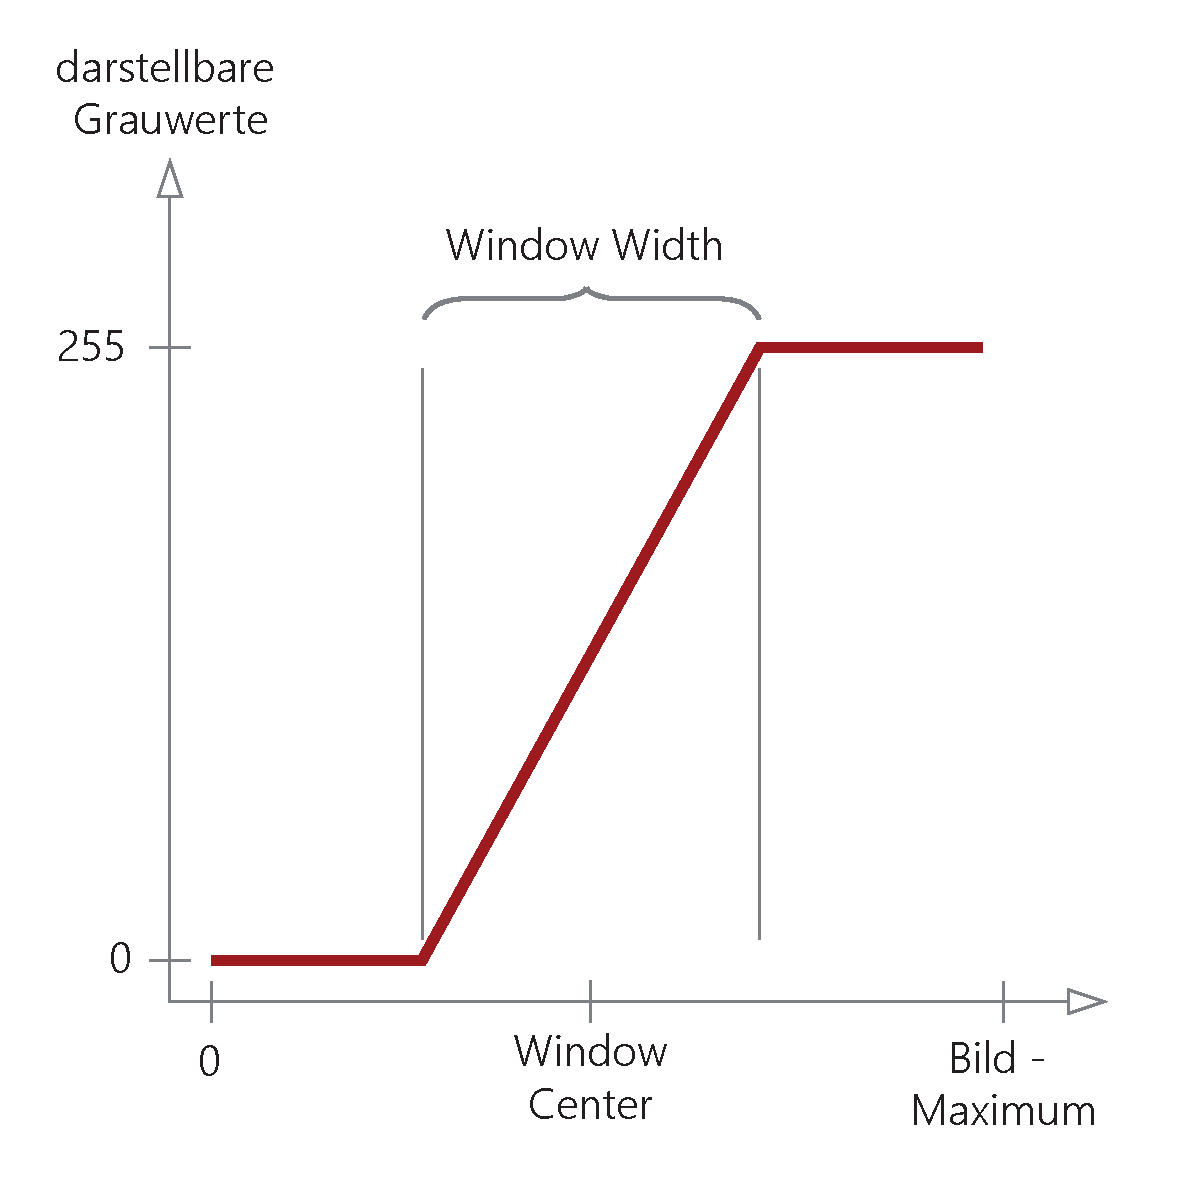
\includegraphics[width=5cm]{./img/fensterung.pdf} \label{window_graph}}
\subfigure[Window Center 50; Window Width 350]{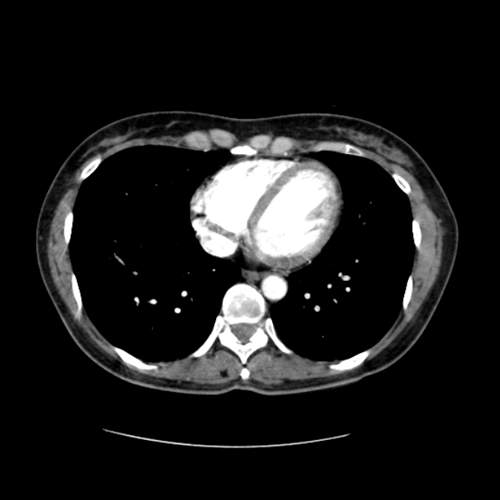
\includegraphics[width=5cm]{./img/window_a.png} \label{window_a}}
\subfigure[Window Center -124; Window Width 3134]{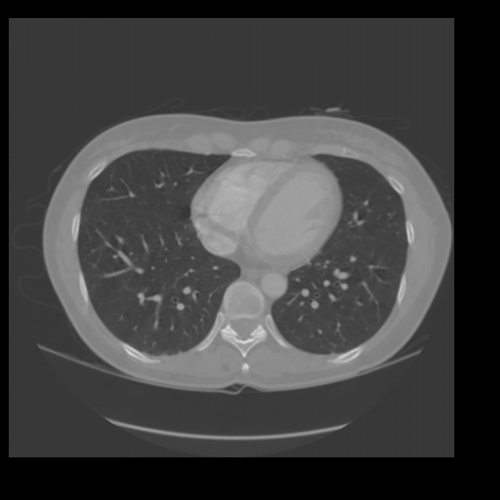
\includegraphics[width=5cm]{./img/window_b.png} \label{window_b}}
}
\floatfoot{Vorlage für die Grafik der Fensterungstechnik ist\cite[Abbildung 8.1]{handels:mbv}; Die Beispieldaten stammen von http://www.osirix-viewer.com/datasets/ - abgerufen am 19.01.2014}
\caption{Fensterungstechnik zur Darstellung medizinischer Bilddaten am handelsüblichen Monitor}
\label{window_sub}
\end{figure*}

\subsection{Farbbilder} \label{color_images}
Obwohl Grauwertbilder das am meisten verwendete Format in der medizinischen Bildverarbeitung darstellen, haben auch Farbbilder die verschiedensten Einsatzgebiete. So wird in der Dermatologie auf Farbdarstellungen zurückgegriffen um Hauterkrankungen zu dokumentieren\cite[2.2.3.2]{handels:mbv}. Des weiteren kann mit Farbultraschallbildern die Fließrichtung und Geschwindigkeit des Blutes visualisiert werden und dienen zur Untersuchung von Venen und Arterien\footnote{http://www.diagnostikum-berlin.de/farbkodierte-duplexsonographie-fkds - abgerufen am 19.01.2014}.\\
Wie bereits beschrieben, ist das Datenelement SamplesPerPixel mit einem Wert von drei der Indikator, dass ein Farbbild vorliegt. Das bedeutet pro Pixel werden 3 Elemente von PixelData belegt mit je einem Element für den roten, grünen und blauen Farbkanal. Daraus resultiert der dreifach Speicherbedarf, $BitsAllocated * SamplesPerPixel$ \cite[C.7.6.3.1.1]{dicom:iod}. Der DICOM-Standard bietet zwei Möglichkeiten, wie diese Information im Speicher hinterlegt werden. Entweder werden die Pixelwerte fortlaufend gespeichert mit R1, G1, B1; R2 ,G2, B2; ...RN, GN, BN; oder nach dem Kanal R1, R2, ...RN; G1, G2, ...GN; B1, B2, ...BN \cite[C.7.6.3.1.3]{dicom:iod}. Das Element dazu aus dem Data Dictionary heißt PlanarConfiguration(0028,0006). Abbildung \ref{planar} macht die beiden Schemata deutlich.

\begin{figure*}[htb]
%\subfigure[Keypoints]{\includegraphics[width=0.49\textwidth]{./img/basmati_keypoints.png}}\hfill
\centering
\fbox{
\subfigure[PlanarConfiguration = 0]{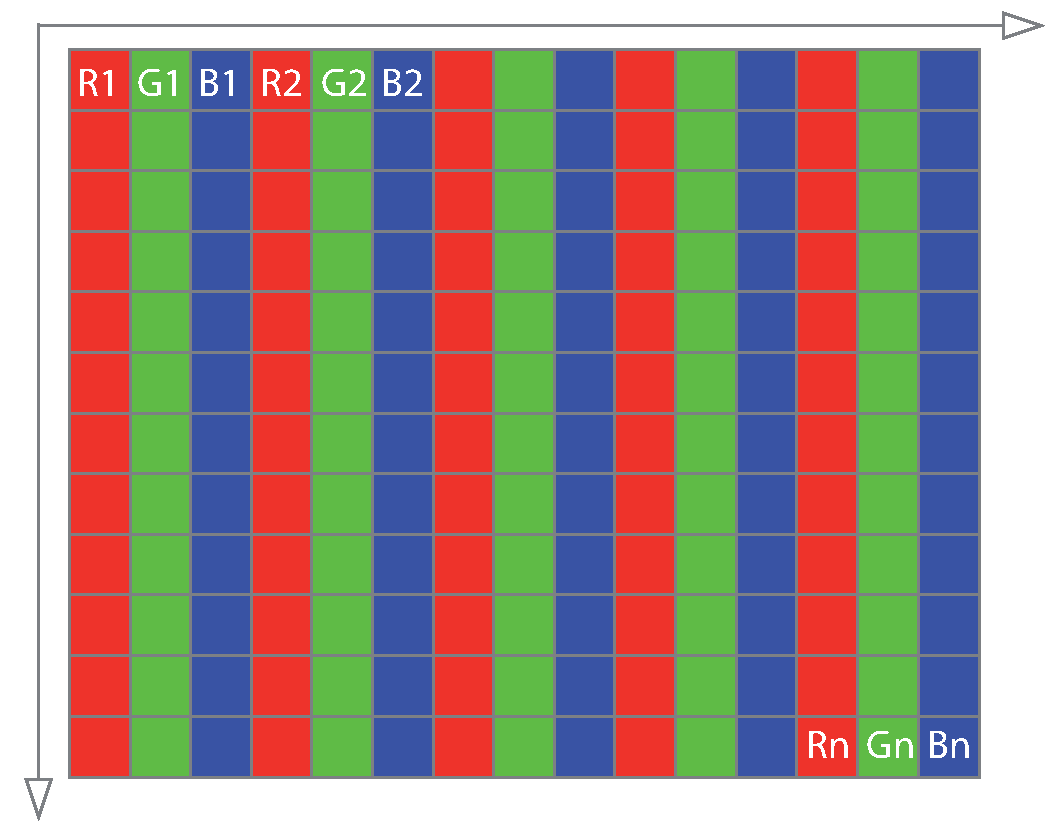
\includegraphics[width=8cm]{./img/planar_b.pdf} \label{planar_a}}
\subfigure[PlanarConfiguration = 1]{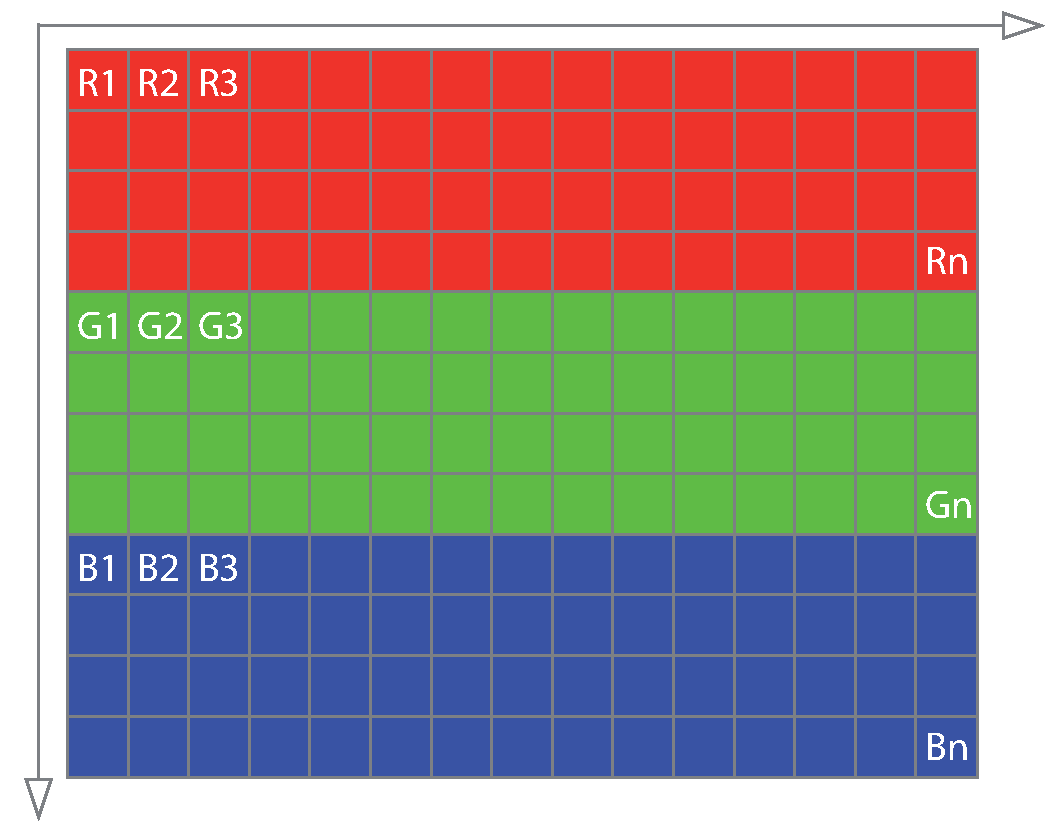
\includegraphics[width=8cm]{./img/planar_a.pdf} \label{plaanr_b}}
}
%\floatfoot{Vorlage für die Grafik der Fensterungstechnik ist\cite[Abbildung 8.1]{handels:mbv}; Die Beispieldaten stammen von http://www.osirix-viewer.com/datasets/ - abgerufen am 19.01.2014}
\caption{Kodierung der RGB-Werte im Datenelement PixelData mit Hilfe der PlanarConfiguration}
\label{planar}
\end{figure*}

\section{3D Bilddaten}
Sowohl die Grauwertdarstellungen, als auch Farbbilder wurden bisher nur als eine zweidimensionale Abbildung behandelt. Computertomographen und Magnetresonanztomographen sind in der Lage Schichten des menschlichen Körpers aufzunehmen. Die Menge der Schichtaufnahmen stellen eine Serie dar (vgl.\nameref{grundlagen:iod} \pageref{grundlagen:iod}). Durch die Verbindung der einzelnen DICOM-Objekte wird der Pixelraum verlassen und der Voxelraum betreten. Ein Voxel ist die dreidimensionale Repräsentation eines Pixels, mit der Tiefe als zusätzliche Dimension zu Breite und Höhe.

\begin{figure*}[htb]
%\subfigure[Keypoints]{\includegraphics[width=0.49\textwidth]{./img/basmati_keypoints.png}}\hfill
\centering
\fbox{
\subfigure[2D Darstellung]{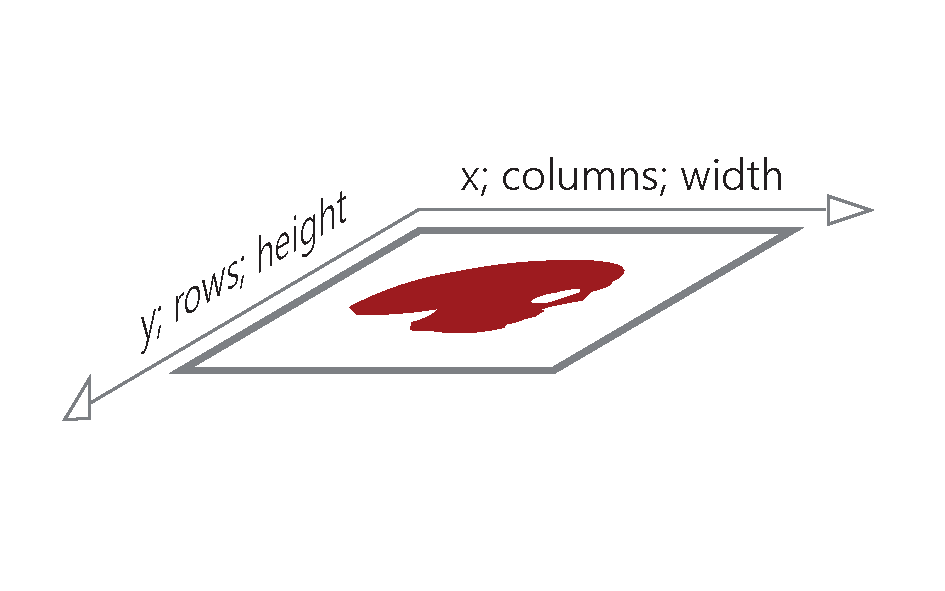
\includegraphics[width=5cm]{./img/2d.pdf} \label{2d}}
\subfigure[3D Bildfolge]{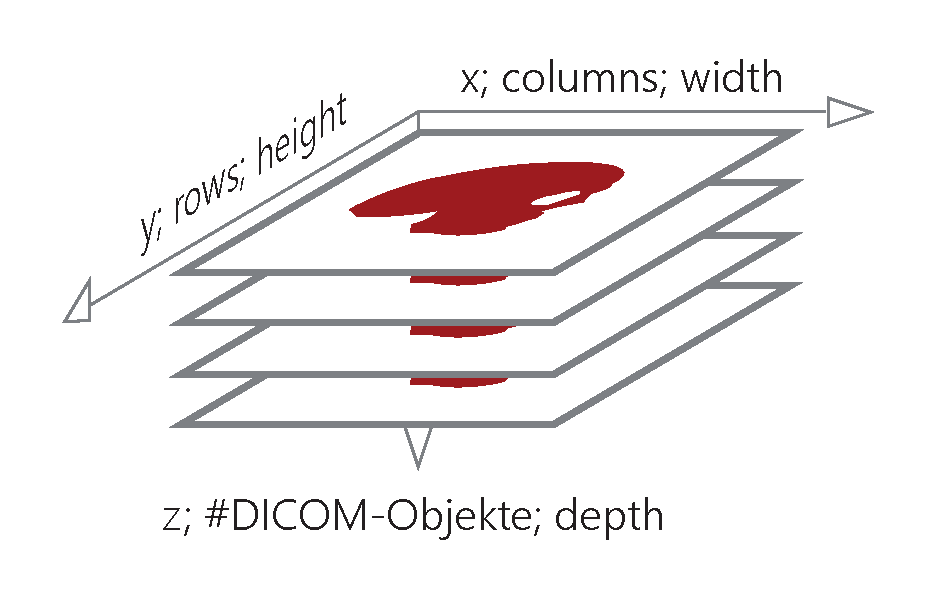
\includegraphics[width=5cm]{./img/3d.pdf} \label{3d}}
\subfigure[zeitlich Abhängige 3D Bildfolge]{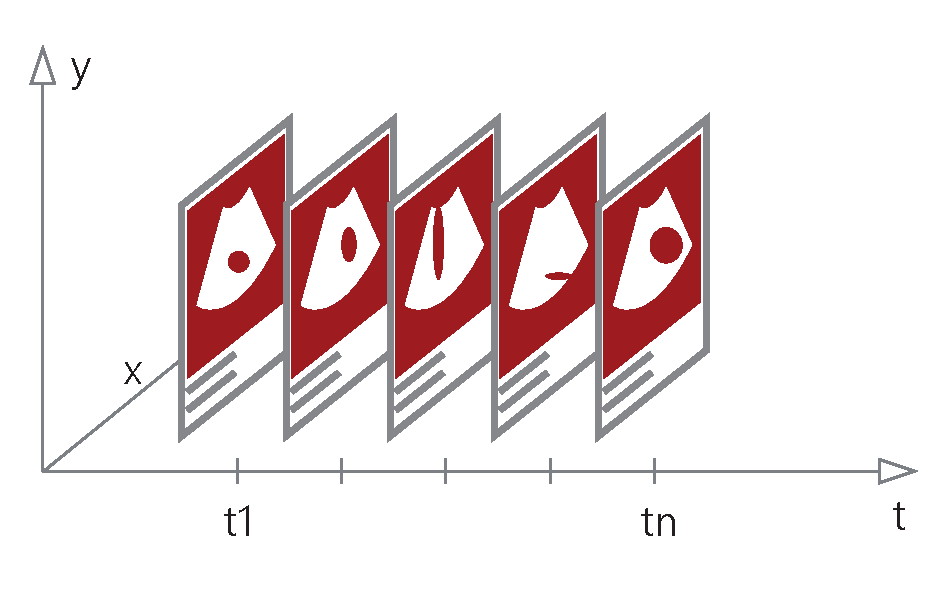
\includegraphics[width=5cm]{./img/time.pdf} \label{time3d}}
}
%\floatfoot{Vorlage für die Grafik der Fensterungstechnik ist\cite[Abbildung 8.1]{handels:mbv}; Die Beispieldaten stammen von http://www.osirix-viewer.com/datasets/ - abgerufen am 19.01.2014}
\caption{Darstellung von 2- und 3-dimensionalen Bilddaten}
\label{dimensions}
\end{figure*}

\section{Bilder mit zeitlicher Abhängigkeit}

Auch Bildaufnahmen zu verschiedenen Zeitpunkten sind dreidimensionale Bildfolgen, wobei die Zeit die dritte Dimension darstellt\cite[2.2.5]{handels:mbv}. Häufige Einsatzgebiete für Bewegtbildfolgen ist die Endoskopie oder Sonographie. Die Abbildung \ref{time3d} macht den Unterschied zwischen zeitlicher und räumlicher Dimension deutlich. Räumliche Darstellungen sind grundsätzlich in mehrere DICOM-Objekte und Dateien aufgeteilt. Zeitlich abhängige Daten sind in einem einzigen Objekt zusammengefasst. NumberOfFrames (0028,0008) gibt die Anzahl an unterschiedlichen Aufnahmen und Zeitpunkten an, die in PixelData enthalten sind.

\chapter{Implementierung} \label{implementation}

\section{Module}


\pagebreak

\setcounter{page}{1}
\renewcommand{\thepage}{\Roman{page}}

%Literatur
%\addcontentsline{toc}{section}{Literaturverzeichnis}
%\setcounter{lofdepth}{2}
\stopthumb
%\bibliographystyle{alpha}
\bibliographystyle{alphadin}  
\bibliography{literature}

%\addcontentsline{toc}{section}{Abbildungsverzeichnis}
\listoffigures
\listoftables

\appendix
\chapter{Darstellung der DICOM-Elemente im Speicher} \label{appendix:speicher}
\section{Explizite VR mit [ OB \textpipe\ OW \textpipe\ OF \textpipe\ SQ \textpipe\ UT \textpipe\ UN ]}

Bei expliziter VR-Struktur besteht das Element aus vier konsekutiven Feldern. Ist die VR vom Typ OB, OW, OF, SQ, UT oder UN wird das Datenelement wie in Tabelle \ref{table:appendix_explizit} im Speicher abgelegt. Die reservierten 2 Byte im VR-Teil sind für zukünftige Weiterentwicklungen des DICOM-Standards.\cite[7.1.2]{dicom:structure}

\begin{sidewaystable}
    \begin{tabularx}{\textwidth}{|X|X|p{5cm}|X|X|p{8cm}|}
    \toprule \hline
   \multicolumn{2}{|l|}{\textbf{Tag}} 	&	\multicolumn{2}{l|}{\textbf{VR}} 		&		\textbf{Value Length}   	& 	\textbf{Value} \\ \hline
    Group \# 16-bit unsigned integer & Element \# 16-bit unsigned integer  &  VR 2-byte character String [OB | OW | OF | SQ | UT | UN ] & Reservierter
    Bereich & 32-bit unsigned integer  &  Gerade Anzahl an Byte. Enthält den Wert des Datenelements. Kodierung abhängig von VT-Typ und Transfersyntax. Wenn die Länge nicht definiert ist wird diese auf \glqq Sequence Delimitation\grqq\ limitiert. \\ \hline
	
	2 Byte & 2 Byte & 2 Byte & 2 Byte & 4 Byte & Anzahl an Byte entsprechend der \glqq Value Length\grqq\, wenn von explizieter Länge \\ \hline
	
	\bottomrule
    \end{tabularx}
    \caption {Darstellung des Datenelements im Speicher wenn VR vom Typ OB, OW, OF, SQ, UT oder UN}
    \label{table:appendix_explizit}
\end{sidewaystable}

\section{Explizite VR}

Diese Darstellung wird gewählt wenn VR \textit{nicht} vom Typ OB, OW, OF, SQ, UT oder UN ist. Der Unterschied besteht im Feld \glqq Value Length\grqq\. Bei der Form von Tabelle \ref{table:appendix_explizit} ist dieses Feld 32 Bit lange. Hier beträgt es lediglich 16 Bit \cite[7.1.2]{dicom:structure}. Der Grund liegt am erhöhten Speicherbedarf von \ref{table:appendix_explizit}, da die Länge des Wertes eine undefinierte Länge haben kann.

\begin{sidewaystable}
	\begin{tabularx}{\textwidth}{|X|X|X|X|p{12cm}|}
	\toprule \hline
	\multicolumn{2}{|l|}{\textbf{Tag}} & \textbf{VR} 2 & \textbf{Value Length} & \textbf{Value} 4 \\ \hline
	Group \# 16-bit unsigned integer & Element \# 16-bit unsigned integer & VR 2-byte character String 2 & 16-bit unsigned integer & Gerade Anzahl an Byte. Enthält den Wert des Datenelements. Kodierung abhängig von VT-Typ und Transfersyntax. \\ \hline
	2 Byte & 2 Byte & 2 Byte & 2 Byte & \glqq Value Length\grqq\ Byte \\ \hline
	\bottomrule
	\end{tabularx}
    \caption {Darstellung des Datenelements für alle anderen VR-Typen}
    \label{table:appendix_explizit_else}
\end{sidewaystable}

\section{Implizite VR}

Bei einer impliziten VR Darstellung besteht das Datenelement aus den drei konsekutive Feldern Tag, Value Length und dem Wert selbst \cite[7.1.3]{dicom:structure}.

\begin{sidewaystable}
	\begin{tabularx}{\textwidth}{|X|X|X|p{12cm}|}
	\toprule \hline
	\multicolumn{2}{|l|}{\textbf{Tag}} & \textbf{Value Length} 2 & \textbf{Value} \\ \hline
	Group \# 16-bit unsigned integer & Element \# 16-bit unsigned integer & 32-bit unsigned integer & Gerade Anzahl an Byte. Enthält den Wert des Datenelements. Kodierung abhängig von VT-Typ spezifiziert in \cite{dicom:dd} und Transfersyntax. Wenn die Länge nicht definiert ist wird diese auf \glqq Sequence Delimitation\grqq\ limitiert. \\ \hline
	2 Byte & 2 Byte & 2 Byte & \glqq Value Length\grqq\ Byte oder undefinierte Länge \\ \hline
	
	\bottomrule
	
	\end{tabularx}
    \caption {Darstellung des Datenelements für implizite VR.}
    \label{table:appendix_implizit}
\end{sidewaystable}



\end{document}